\documentclass[a4paper,12pt]{article}

\usepackage[utf8]{inputenc}

\usepackage[T1]{fontenc}

\usepackage{geometry}

\geometry{a4paper, margin=2.5cm}

\usepackage{amsmath, amssymb, amsfonts}

\usepackage{graphicx}

\usepackage{listings}

\usepackage{xcolor}

\usepackage{hyperref}

\usepackage{enumitem}

\usepackage{booktabs}

\usepackage{fancyhdr}

\usepackage{tikz}



% Colors for code listings

\definecolor{codegreen}{rgb}{0,0.6,0}

\definecolor{codegray}{rgb}{0.5,0.5,0.5}

\definecolor{codepurple}{rgb}{0.58,0,0.82}

\definecolor{backcolour}{rgb}{0.95,0.95,0.92}



\lstdefinestyle{mystyle}{

    backgroundcolor=\color{backcolour},   

    commentstyle=\color{codegreen},

    keywordstyle=\color{magenta},

    numberstyle=\tiny\color{codegray},

    stringstyle=\color{codepurple},

    basicstyle=\ttfamily\footnotesize,

    breakatwhitespace=false,         

    breaklines=true,                 

    captionpos=b,                    

    keepspaces=true,                 

    numbers=left,                    

    numbersep=5pt,                  

    showspaces=false,                

    showstringspaces=false,

    showtabs=false,                  

    tabsize=2

}

\lstset{style=mystyle}



\pagestyle{fancy}

\fancyhf{}

\lhead{MST V4: Drehgeber Lab Prep}

\rhead{WiSe 2025/2026}

\cfoot{\thepage}



\title{\textbf{Preparation Guide: MST V4 - Drehgeber}\\Inductive Sensors \& Signal Processing}

\author{University Lab Assistant}

\date{Winter Semester 2025/2026}



\begin{document}



\maketitle

\tableofcontents

\newpage



\section{Theoretical Foundations \& Test Preparation}



\subsection{Goal of the Experiment}

The objective of this laboratory session is to understand the signal chain of a rotational speed sensor system. The process involves:

\begin{enumerate}

    \item Recording a real analog signal from a passive inductive sensor (Drehgeber).

    \item Digitizing and processing the data in a PC (Excel).

    \item Replicating the signal using an Arbitrary Waveform Generator to simulate specific scenarios (e.g., a missing tooth on a gear).

\end{enumerate}



\subsection{The Inductive Sensor (Passive)}

The experiment uses a Bosch inductive speed sensor (Reference: 0 261 210 104)~\cite{ref25,ref26}.



\subsubsection{Physical Principle}

The sensor operates on the principle of electromagnetic induction (Faraday's Law of Induction). It consists of:

\begin{itemize}

    \item A permanent magnet (Dauermagnet)~\cite{ref13}.

    \item A soft iron core (Weicheisenkern)~\cite{ref16}.

    \item A coil (Spule) with $N$ windings~\cite{ref17}.

\end{itemize}



As a ferromagnetic gear tooth (Zahnscheibe)~\cite{ref19} passes the sensor tip, it changes the magnetic reluctance of the magnetic circuit. This changes the magnetic flux $\Phi$ through the coil.



The induced voltage $U_{ind}$ is given by:

\begin{equation}

    U_{ind} = -N \cdot \frac{d\Phi}{dt}

\end{equation}



\subsubsection{Signal Characteristics}

\begin{itemize}

    \item **Waveform:** Quasi-sinusoidal. The peak occurs at the steepest gradient of the magnetic flux (edge of the tooth). Zero-crossing occurs at the center of the tooth or gap.

    \item **Passive:** It requires no external power supply (Hilfsenergie)~\cite{ref5}. The 2-wire cable carries the signal directly.

    \item **Speed Dependence:**

    \begin{itemize}

        \item \textbf{Frequency ($f$):} Directly proportional to rotational speed ($n$) and number of teeth ($z$).

        \item \textbf{Amplitude ($U_{peak}$):} Also proportional to rotational speed. Since $U \propto \frac{d\Phi}{dt}$, faster rotation means faster flux change, resulting in higher voltage.

    \end{itemize}

\end{itemize}



\subsection{Hall Sensor (Comparison)}

Although the inductive sensor is the focus, a Hall sensor is present in the setup~\cite{ref5}. Unlike the inductive sensor:

\begin{itemize}

    \item It is an **active** sensor (requires power).

    \item It measures the magnitude of the B-field, not the rate of change.

    \item It can detect speed down to 0 RPM (static detection), whereas inductive sensors produce 0V at standstill.

\end{itemize}



\newpage



\section{Worksheet Solutions \& Practical Guide}



\subsection{Task 1: Hardware Setup \& Connection}

\textbf{Instructions:}

\begin{itemize}

    \item Connect the Inductive Sensor output directly to the Oscilloscope (Owon) via BNC.

    \item Power the Motor using the DC power supply.

    \item \textbf{Limit:} Set the power supply to max \textbf{5V} and \textbf{2A}~\cite{ref37}.

\end{itemize}



\begin{figure}[h]

    \centering

    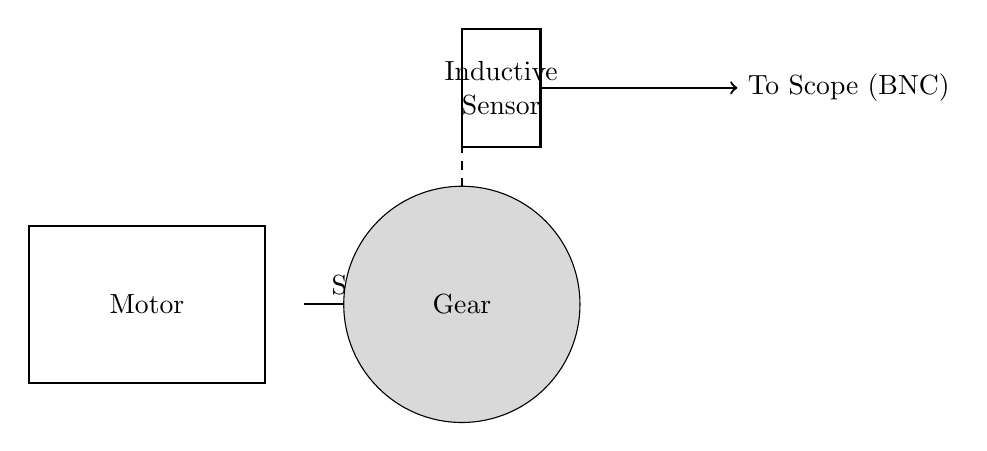
\begin{tikzpicture}

        \draw[thick] (0,0) rectangle (3,2) node[midway] {Motor};

        \draw[thick, ->] (3.5,1) -- (5,1) node[midway, above] {Shaft};

        \draw[fill=gray!30] (5.5,1) circle (1.5);

        \node at (5.5,1) {Gear};

        \draw[thick] (5.5,3) rectangle (6.5,4.5) node[midway, align=center] {Inductive\\Sensor};

        \draw[thick, ->] (6.5,3.75) -- (9,3.75) node[right] {To Scope (BNC)};

        \draw[thick, dashed] (5.5, 2.5) -- (5.5, 3);

    \end{tikzpicture}

    \caption{Simplified Setup Diagram}

\end{figure}



\subsection{Task 2: Excel Evaluation \& Calculations}

\textbf{Scenario:} You have recorded the CSV data from the Owon oscilloscope.



\subsubsection{A. Determining Frequency ($f$)}

1. Identify the period $T$ (time for one full sine wave).

2. Use the formula:

\begin{equation}

    f = \frac{1}{T}

\end{equation}

\textit{Example from data:} If one period spans $16 \text{ms}$ ($0.016 \text{s}$):

$$ f = \frac{1}{0.016} = 62.5 \text{ Hz} $$



\subsubsection{B. Determining Rotational Speed (RPM)}

The relationship between signal frequency and mechanical speed is:

\begin{equation}

    f = \frac{n \cdot z}{60} \implies n = \frac{f \cdot 60}{z}

\end{equation}

Where:

\begin{itemize}

    \item $n$ = Speed in revolutions per minute (RPM).

    \item $z$ = Number of teeth on the gear. (Assume $z=60$ if not specified, or count peaks per one motor revolution if the motor speed is known).

    \item $f$ = Measured frequency (Hz).

\end{itemize}



\subsubsection{C. Frequency and Amplitude vs. Speed~\cite{ref42}}

\textbf{Question:} How do frequency and amplitude change with speed?

\textbf{Answer:}

\begin{itemize}

    \item \textbf{Frequency:} Increases linearly with speed ($f \sim n$).

    \item \textbf{Amplitude:} Increases linearly with speed ($U_{ind} \sim n$). At higher speeds, the change in magnetic flux $d\Phi/dt$ is larger.

\end{itemize}



\subsection{Task 3: Arbitrary Signal Generation (The "Missing Tooth")}

\textbf{Goal:} Modify the CSV data to remove 4 teeth (simulate a gap) and replay it~\cite{ref182}.



\textbf{Why?} In automotive applications (e.g., crankshafts), a "60-2" or similar gap is used to determine the \textit{absolute} position (Top Dead Center) of the engine, not just the speed.



\textbf{Procedure:}

1. Open `SchreibeRigolRaf.xlsm`.

2. Paste your voltage data into the appropriate column.

3. Locate 4 consecutive sine waves (periods).

4. Set their voltage values to 0 (or near 0) to simulate the air gap.

5. Generate the `.raf` file using the macro button.



\textbf{Code Logic (Python Equivalent for understanding):}

\begin{lstlisting}[language=Python, caption=Simulating Missing Tooth Logic]

import numpy as np



# Assume data is an array of voltage values

voltage_data = load_csv("scope_data.csv")



# Identify indices to zero out (e.g., index 100 to 140 representing 4 periods)

start_gap = 100

end_gap = 140



# Apply the gap (Missing Tooth)

voltage_data[start_gap:end_gap] = 0.0 



# This modified array is then sent to the Arbitrary Waveform Generator

save_raf_format(voltage_data)

\end{lstlisting}



\subsection{Task 4: Signal Replay (Rigol Setup)}

Depending on the generator model (DG 4062 or DG 1022)~\cite{ref211,ref224}:

\begin{enumerate}

    \item Press **Arb** button.

    \item Insert USB stick (formatted FAT16, max 4GB recommended)~\cite{ref186}.

    \item Navigate: `Store/Recall` or `Select Wform` $\rightarrow$ `External/UDisk`.

    \item Load the `.raf` file.

    \item \textbf{Important:} Enable the **Output** button to see the signal on the scope.

\end{enumerate}



\newpage



\section{Further Questions \& Glossary}



\subsection{Review Questions}

\begin{enumerate}

    \item \textbf{Q: Why does the inductive sensor output 0V when the motor stops?}

    \textbf{A:} Induction requires a \textit{change} in magnetic flux ($d\Phi/dt$). If there is no movement, $dt \to \infty$, so voltage is zero.



    \item \textbf{Q: How would a Hall sensor's signal differ at low speeds?}

    \textbf{A:} A Hall sensor would still output a distinct High or Low logic level corresponding to whether it is facing a tooth or a gap, even at 0 RPM.



    \item \textbf{Q: Why did we format the USB stick to FAT16?}

    \textbf{A:} Older measurement equipment (like the Rigol generators) often requires simple file systems and has capacity limits (e.g., 4GB) to recognize the drive~\cite{ref187}.



    \item \textbf{Q: If we double the number of teeth $z$, what happens to the frequency at the same RPM?}

    \textbf{A:} The frequency doubles ($f \propto z$).



    \item \textbf{Q: Why is the "Missing Tooth" signal useful for ECU testing?}

    \textbf{A:} It allows engineers to test Engine Control Units (ECUs) in a lab environment without running a real engine, verifying if the ECU correctly identifies Top Dead Center (TDC) via the gap.

\end{enumerate}



\subsection{Formula Sheet}

\begin{table}[h]

    \centering

    \begin{tabular}{@{}ll@{}}

    \toprule

    \textbf{Parameter} & \textbf{Formula} \\ \midrule

    Induction Law & $U_{ind} = -N \frac{d\Phi}{dt}$ \\

    Frequency & $f = \frac{1}{T}$ \\

    RPM (Drehzahl) & $n = \frac{f \cdot 60}{z}$ \\

    Angular Velocity & $\omega = 2\pi f$ \\ \bottomrule

    \end{tabular}

    \caption{Key Formulas}

\end{table}



\subsection{Glossary}

\begin{itemize}

    \item \textbf{Drehgeber:} Rotary Encoder. A sensor to measure rotation speed or position.

    \item \textbf{Inductive Sensor:} Passive sensor using magnetic coil.

    \item \textbf{Luftspalt (Air Gap):} Distance between sensor tip and gear tooth. Smaller gap = Stronger signal.

    \item \textbf{Bezugsmarke:} Reference mark (e.g., the missing tooth) for absolute positioning.

    \item \textbf{Arbitrary Waveform:} A user-defined signal shape, not just standard sine/square waves.

\end{itemize}



\newpage

\section*{References}

\begin{thebibliography}{99}

\bibitem{ref5} Hall sensor comparison and passive sensor characteristics.

\bibitem{ref13} Permanent magnet (Dauermagnet) in inductive sensors.

\bibitem{ref16} Soft iron core (Weicheisenkern) components.

\bibitem{ref17} Coil windings in inductive sensors.

\bibitem{ref19} Ferromagnetic gear tooth (Zahnscheibe) interaction.

\bibitem{ref25} Bosch inductive speed sensor reference 0 261 210 104.

\bibitem{ref26} Bosch inductive speed sensor specifications.

\bibitem{ref37} Power supply limits: 5V and 2A maximum.

\bibitem{ref42} Frequency and amplitude relationship with speed.

\bibitem{ref182} Missing tooth simulation procedure.

\bibitem{ref186} USB stick formatting requirements (FAT16, 4GB limit).

\bibitem{ref187} File system compatibility for measurement equipment.

\bibitem{ref211} Rigol DG 4062 arbitrary waveform generator.

\bibitem{ref224} Rigol DG 1022 arbitrary waveform generator.

\end{thebibliography}



\end{document}

